
\chapter*{Multiengine Airplanes:\\An Introduction}

%\begin{center}
%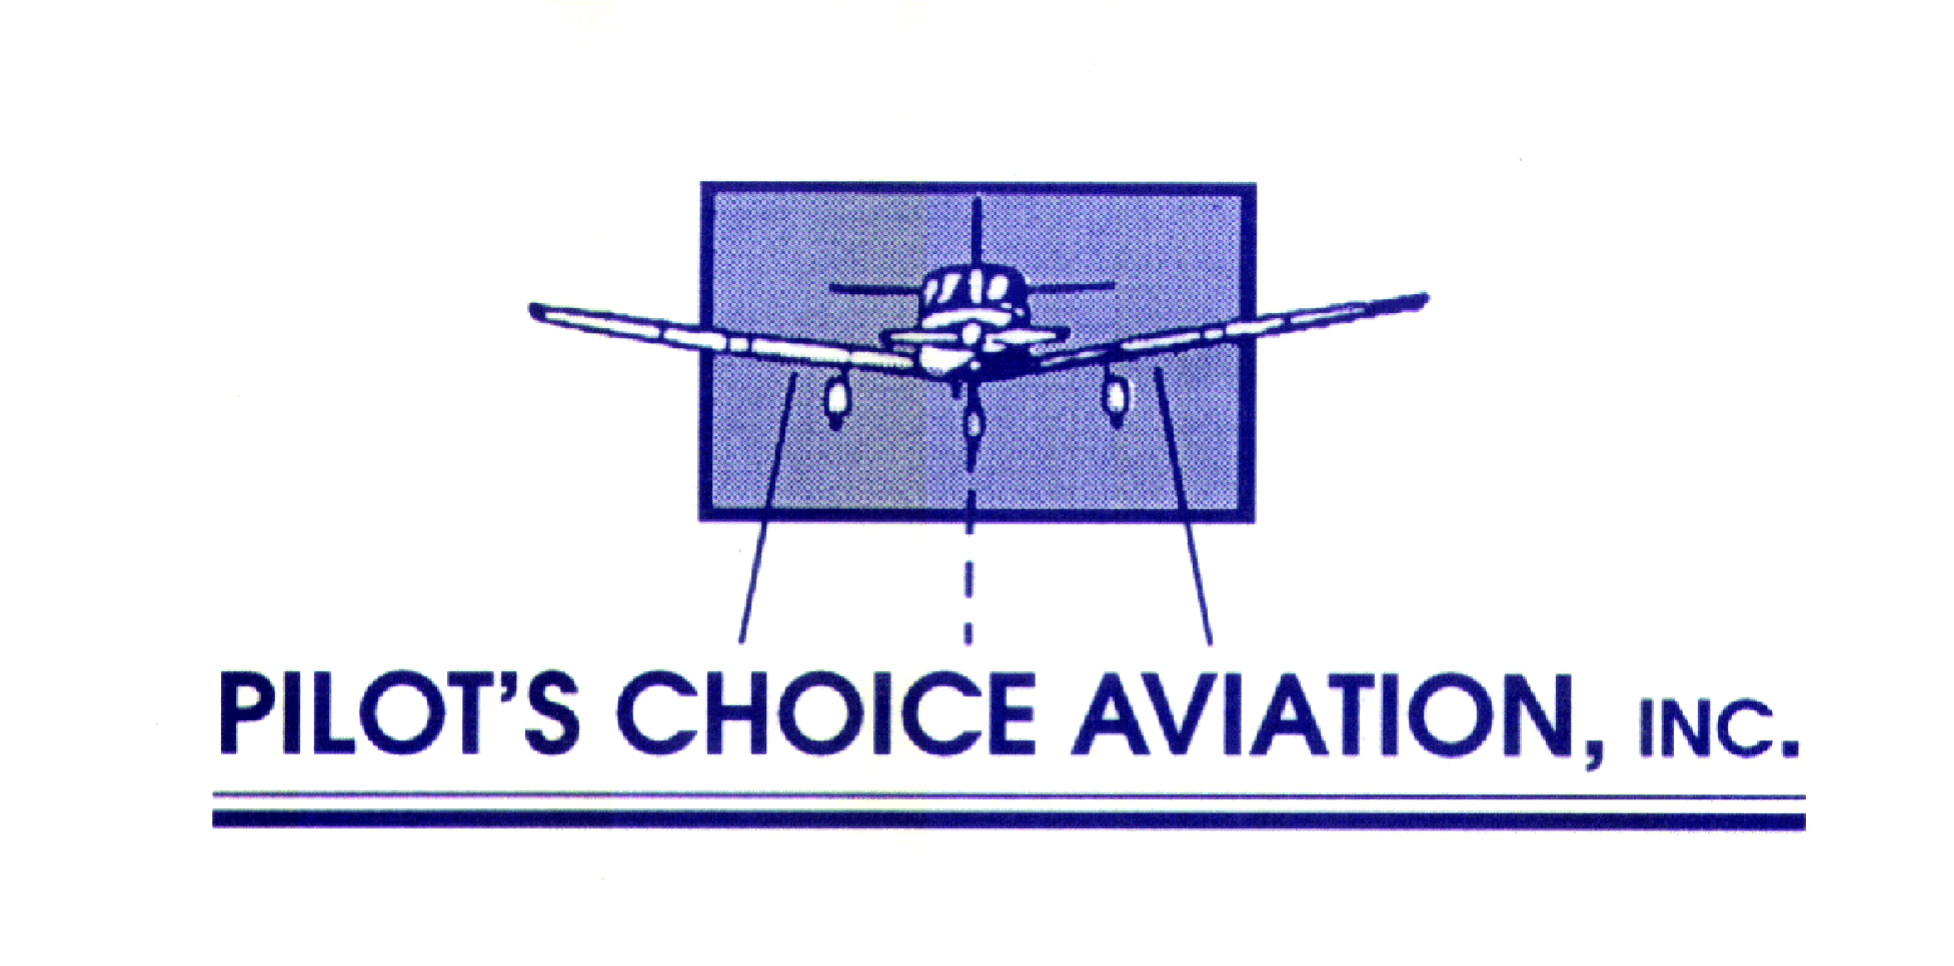
\includegraphics[width=0.9\linewidth]{pca-logo.png}
%\end{center}

Do you want to fly the ``big iron''? Are you looking for more performance, capability,
and reliability? Do you enjoy engine management (and maintenance) so much that you want to
double the fun? Do you see a type rating in your future? If so, multi engine airplane training is for you.


This Manual focuses on the Beechcraft Duchess BE-76, a popular multiengine trainer.
%used at Pilot's Choice Aviation, Inc. (PCA) at Georgetown, TX (KGTU).

The material in this book is based upon official resources from the FAA, as well as Beechcraft.

Beth Ann Jenkins and Stephanie Fernihough of Pilot's Choice Aviation, Inc., Georgetown, TX
wrote an earlier version of this manual, with the assistance of many others over the years.

Jos\'e reformatted the Multiengine Manual \LaTeX{} in Spring of 2025. At that time, it was also
updated to include notes eight years of students successfully using this document to become multi
engine pilots. System diagrams were upgraded to new, higher quality vector graphics. This Manual
contains updated material the latest FAA ACS testing documents as of this writing.
%
%\newpage

\section*{Disclaimer}

The information contained in this publication is subject to change.

Aeronautical information, regulations, and aircraft information change regularly, therefore those relevant
publications should be referred to for any critical information.

The information in this manual is to be utilized for training purposes only. Always
refer to your aircraft's POH, AFM, and other certified documentation before flight!
